\providecommand{\main}{..}
\documentclass[\main/main.tex]{subfiles}
\begin{document}
\chapter{Note per lo studio}
\section{Mappa mentale}
\begin{figure}
	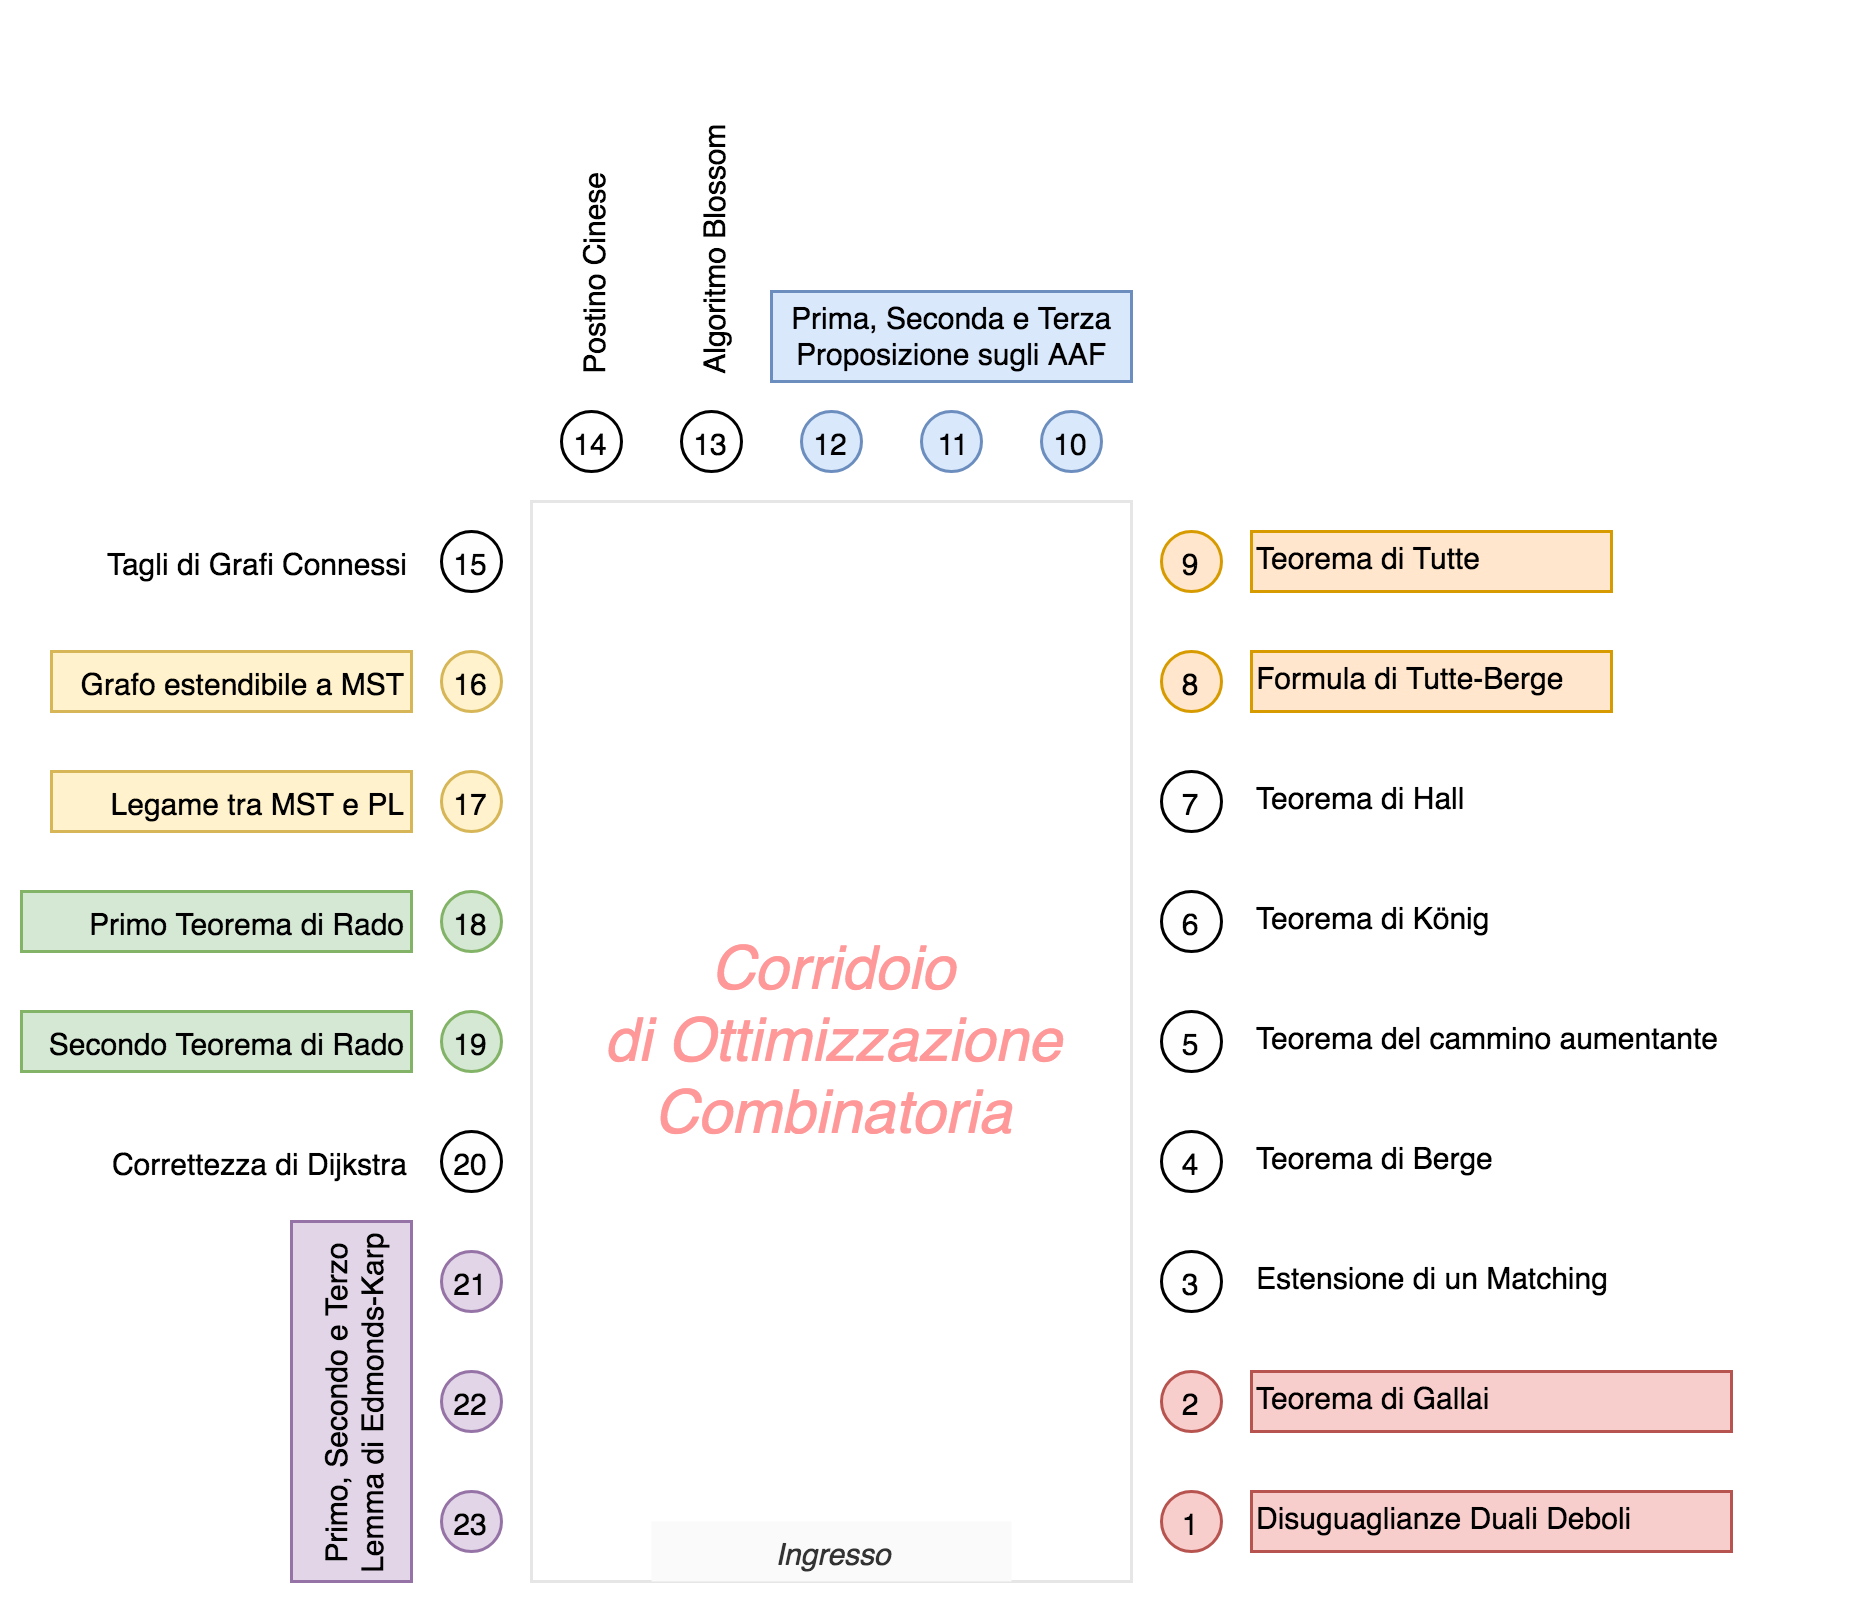
\includegraphics[width=\textwidth]{map}
\end{figure}
\clearpage
\section{Sinossi dei teoremi}
\begin{multicols}{2}
	\begin{description}
		\item[Disuguaglianze Duali Deboli] Identifica un legame di disuguaglianza tra la cardinalità di \textbf{insieme stabile massimo} ed \textbf{edge cover minimo} e tra cardinalità di \textbf{matching massimo} ed \textbf{insieme trasversale minimo}.
		\item[Teorema di Gallai] Identifica un legame di uguaglianza tra somma delle cardinalità di \textbf{insieme stabile massimo} ed \textbf{insieme trasversale minimo} ed il numero di nodi \(n\) nel grafo. Inoltre, se non esistono nodi isolati, identifica anche un secondo legame tra la somma delle cardinalità del \textbf{matching massimo} ed l'\textbf{edge cover minimo} ed il numero di nodi del grafo.
		\item[Estensione di un Matching] Partendo da un matching \(M\) noto, definisce un modo per trovare un matching \(M'\) di cardinalità \(\abs{M}+1\) utilizzando un cammino aumentante.
		\item[Teorema di Berge] Un matching è massimo solo se non esiste un matching a cardinalità maggiore, che si può identificare tramite un cammino aumentante. Di conseguenza, un matching è massimo solo se non esistono aggiuntivi cammini aumentanti e viceversa.
		\item[Teorema del Cammino Aumentante] Definisce un vincolo di appartenenza di un vertice esposto al matching massimo se non è possibile costruire un cammino aumentante che parte da esso per un qualsiasi matching \(M\) per cui il vertice è esposto.
		\item[Teorema di König] Identifica una uguaglianza tra cardinalità del \textbf{matching massimo} ed \textbf{insieme trasversale minimo} quando il grafo su cui sono definiti è \textbf{bipartito}.
		\item[Teorema di Hall] In un \textbf{grafo bipartito} esiste un \textbf{matching massimo} se e solo se ogni vertice della componente minore ha almeno un vertice incidente distinto della componente maggiore.
		\item[Formula di Tutte-Berge] Definisce la dimensione del matching massimo di un grafo in funzione del numero di componenti connesse del grafo con vertici dispari.
		\item[Teorema di Tutte] Identifica una condizione di esistenza di un \textbf{matching perfetto} in un grafo basata sul numero di componenti connesse dispari in tutti i suoi sottoinsiemi di nodi.
		\item[Albero alternante frustrato] Un albero alternante in un grafo \(\Gr \) si dice frustrato se ogni lato di \(G\) avente un termine in \(B(T)\) possiede l'altro termine in \(A(T)\).
		\item[Prima proposizione sugli AAF] Un grafo con un matching \(M\) ed un AAF associato non può avere un \textbf{matching perfetto}.
		\item[Seconda proposizione sugli AAF] Un grafo con un matching \(M\) ed un albero \(M\)-alternante non può avere un \textbf{matching perfetto} perché un albero così costruito è un AFF.
		\item[Terza proposizione sugli AAF] Se in un albero \(T'\) \(M'\)-alternante definito su di un matching \(M'\) tratto da un grafo \(G'\) derivato da \(G\) non vi sono pseudo-nodi nell'insieme \(A\rnd{T'}\) e l'albero \(T'\) è frustrato allora \(G\) \textbf{non ammette un matching perfetto}.
		\item[Algoritmo Blossom] L'algoritmo determina correttamente se un grafo \(G\) ammette o meno un matching perfetto.
		\item[Algoritmo Ungherese] Si tratta di un algoritmo che determina in tempo polinomiale assegnamenti pesati su grafi bipartiti.
		\item[Problema del Postino Cinese] Problema di trovare un percorso chiuso su grafo pesato di lunghezza minima che contiene un lato di \(G\) almeno una volta.
		\item[Tagli su grafo connesso] Non esiste una partizione del grafo a cui non arrivano archi.
		\item[Grafo estendibile a MST] Definisce una condizione con cui identificare un lato \(e\) da un grafo \(G\) con cui è possibile aumentare un sottografo \(B\subseteq G\) estendibile a MST in modo tale che il grafo aumentato sia a sua volta estendibile a MST.
		\item[Legame tra MST e programmazione lineare] Definisce come sia possibile usare il vettore dei costi di un MST come soluzione ottima di un problema di programmazione lineare.
		\item[Matroide] Un SI che gode della proprietà del primo teorema di Rado \ref{primo_rado} si dice \textbf{matroide}.
		\item[Primo Teorema di Rado] Definisce una identità definita su cardinalità di insiemi indipendenti che se valida per un sistema di indipendenza garantisce che GREEDSUM dia una soluzione ottima per qualsiasi funzione di valutazione.
		\item[Secondo Teorema di Rado] Se per qualsiasi funzione di valutazione GREEDSUM da la soluzione ottima, allora il sistema di cardinalità su cui è definito rispetta l'identità del \textbf{primo teorema di Rado}.
		\item[Correttezza di Dijkstra] Dimostra che Dijkstra identifica un cammino minimo su grafo pesato tra due nodi dati.
		\item[Prima Lemma di Edmonds-Karp] La lunghezza dei cammini passanti dalla sorgente ad ogni nodo e dal ogni nodo alla destinazione da una iterazione alla successiva, aumenta o rimane uguale.
		\item[Secondo Lemma di Edmonds-Karp] Un arco \(e \in E\) cambia stato (usato ed inutilizzato) al più \(\frac{n}{2}\) volte.
		\item[Terzo Lemma di Edmonds-Karp] L'algoritmo di Edmonds-Karp ha complessità \(O\rnd{nm^2}\).
	\end{description}
\end{multicols}

\section{Relazioni e formule importanti}
\begin{figure}
	\begin{subfigure}{0.49\textwidth}
		\begin{align*}
			\a(G)  & \leq \rho(G) \\
			\mu(G) & \leq \tau(G)
		\end{align*}
		\caption{Disuguaglianze Duali Deboli}
	\end{subfigure}
	\begin{subfigure}{0.49\textwidth}
		\begin{align*}
			\a(G) + \tau(G) = n \\
			\mu(G) + \rho(G) = n
		\end{align*}
		\caption{Teorema di Gallai}
	\end{subfigure}
	\begin{subfigure}{0.49\textwidth}
		\[
			M' = \rnd{M\setminus P} \cup \rnd{P\setminus M}
		\]
		\caption{Estensione di un Matching}
	\end{subfigure}
	\begin{subfigure}{0.49\textwidth}
		\[
			\mu\rnd{G} = \tau\rnd{G}
		\]
		\caption{Teorema di König}
	\end{subfigure}
	\begin{subfigure}{0.49\textwidth}
		\[
			\abs{\Gamma(J)} \geq \abs{J} \quad \forall J \subset V_2
		\]
		\caption{Teorema di Hall}
	\end{subfigure}
	\begin{subfigure}{0.49\textwidth}
		\[
			\frac{1}{2} \min_{U \subseteq V} \crl{\abs{U} - \text{odd}\rnd{G-U} + \abs{V}}
		\]
		\caption{Formula di Tutte-Berge}
	\end{subfigure}
	\begin{subfigure}{0.49\textwidth}
		\[
			\text{odd}\rnd{G\setminus A} \leq \abs{A} \quad \forall A \subseteq G
		\]
		\caption{Teorema di Tutte}
	\end{subfigure}
	\begin{subfigure}{0.49\textwidth}
		\[
			\exists I, J \in \rnd{E, F}: \abs{I} = \abs{J} + 1 \quad \exists e \in I: J \cup \crl{e} \in F
		\]
		\caption{Primo Teorema di Rado}
	\end{subfigure}
	\begin{subfigure}{0.49\textwidth}
		\[
			\forall v \in \N, \quad d_{x'}\rnd{s, v} \geq d_{x}\rnd{s, v} \quad \land \quad d_{x'}\rnd{v, t} \geq d_{x}\rnd{v, t}
		\]
		\caption{Primo Lemma di Edmonds-Karp}
	\end{subfigure}
	\caption{Relazioni e formule importanti}
\end{figure}

\end{document}